\documentclass{beamer}

\usepackage[OT4]{fontenc}
\usepackage[utf8]{inputenc}

\author[Łukasz Stolcman]{}
%\subject{Dekoder sygnału wzorca czasu DCF77 z~wykorzystaniem radia programowalnego i~FPGA}

%\usetheme{Warsaw}
\usetheme{Madrid}


%\usetikzlibrary{mindmap,trees}

%\usepackage{listings}
%\lstset{basicstyle=\footnotesize\ttfamily}

\title[Praca inżynierska -- prezentacja]{Dekoder sygnału wzorca czasu DCF77 z~wykorzystaniem radia programowalnego i~FPGA}
\institute[WIZUT]
{
	Zachodniopomorski Uniwersytet Technologiczny w Szczecinie \\
	Wydział Informatyki \\[2cm]
	Łukasz Stolcman
}

\date[Szczecin, 2016]{}



\begin{document}
\begin{frame}
	\titlepage
\end{frame}

\begin{frame}{Spis treści}
	\tableofcontents
\end{frame}

\section{Cele pracy}
\begin{frame}{Cele pracy}

	\begin{exampleblock}{Główny cel}
		Analiza, opracowanie i symulacja prototypu systemu radia programowalnego
	\end{exampleblock}

	\begin{itemize}
		\item \textbf{Sprzęt:} Zaprojektowanie alternatywnej do istniejących platformy SDR
		\item \textbf{Oprogramowanie:} Analiza i implementacja podstawowych modułów
		\item \textbf{Algorytm:} Implementacja jednego z istniejących algorytmów używanych w radiu programowalnym
		\item \textbf{Symulacja:} Symulacja działania zaimplementowanego algorytmu
	\end{itemize} 
\end{frame}

\begin{frame}{Struktura projektu}
	\begin{center}
		\scalebox{0.50}
		{\includegraphics{images/allModules}}
	\end{center}
\end{frame}

\section{Sprzęt}
\begin{frame}{Moduły sprzętowe}

	\begin{itemize}
		\item \textbf{Antena:} dobierana przez użytkownika, sygnał odporowadzany przez złącze BNC
		\item \textbf{Filtry wejściowe:} pasywny filtr eliptyczny
		\item \textbf{Przedwzmacniacz:} LTC6405, Linear Technology
		\item \textbf{ADC:} LTC2208, Linear Technology
		\item \textbf{Zasilanie:} ON NCP1117, TI TPS73733
	\end{itemize} 
\end{frame}

\begin{frame}{PCB - Płytka drukowana}
	\begin{center}
		\scalebox{0.26}
		{\includegraphics{images/pcb-physical}}
	\end{center}
\end{frame}

\section{Moduły programowe}
\begin{frame}{Architektura programowa}
	\begin{center}
		\scalebox{0.43}
		{\includegraphics{images/swModules}}
	\end{center} 
\end{frame}

\begin{frame}{Algorytm Goetzela}
	\begin{center}
		\scalebox{0.43}
		{\includegraphics{images/dcfCarrierEnvelope}
		\includegraphics{images/dcfMinuteMark}}
	\end{center} 
\end{frame}

\section{Symulacje}
\begin{frame}{Symulacje}
	\begin{block}{ModelSim}
		Skrypty symulacyjne przepływu danych w filtrze i~~algorytmie Goertzla
	\end{block}
	\scalebox{0.40}
	{\includegraphics[trim={0 0 15cm 0},clip]{images/sim-goertzel-result}}
\end{frame}

\begin{frame}{Symulacje}
	\begin{block}{Python}
		Skrypt dekodujący komunikat DCF77
	\end{block}
	\scalebox{0.40}
	{\includegraphics[trim={0 0 20cm 0},clip]{images/sim-find}}
\end{frame}

\section{Rezultaty}
\begin{frame}{Rezultaty}
	\begin{itemize}
		\item Prototyp PCB działa
		\item Zasoby FPGA wystarczające do syntezy projektu
		\item Symulacje oprogramowania zakończone powodzeniem
		\item Możliwość dalszego rozwoju algorytmów w FPGA
	\end{itemize} 
\end{frame}

\begin{frame}{Dalszy rozwój}
	\begin{itemize}
		\item \textbf{Sprzęt}: Opracowanie wersji finalnej, usunięcie błędów
		\item \textbf{Oprogramowanie}: Napisanie zoptymalizowanej wersji algorytmów
		\item \textbf{Interfejsy}: Dodanie szybkich interfejsów typu Ethernet oraz dla popularnych programów typu GNU Radio
		\item \textbf{Rzeczywiste uruchomienie}: Testowanie projektu w rzeczywistym środowisku
	\end{itemize} 
\end{frame}

\begin{frame}
	\begin{center}
		Dziękuję za uwagę
	\end{center}
\end{frame}


\end{document}



